\documentclass[a4paper, 12pt]{article}
\usepackage[utf8]{inputenc}
\usepackage[lmargin=3cm, tmargin=3cm, rmargin=2cm, bmargin=2cm]{geometry}
\usepackage[onehalfspacing]{setspace}
\usepackage[T1]{fontenc}
\usepackage[brazil]{babel}

%%%\usepackage{amssymb, amsmath, mathptmx}%bigominus

\usepackage{wasysym}%male and female

\usepackage{graphicx, graphics, xcolor, comment, enumerate, multirow, multicol, indentfirst}

\usepackage{amsmath, amsthm, amsfonts, amssymb, dsfont, mathtools}
\everymath{\displaystyle} 

\usepackage{blindtext}

\usepackage[round]{natbib}
\bibliographystyle{apalike}

%Code packages:
\usepackage{listings}
\usepackage{xcolor}

%New colors defined below
\definecolor{codegreen}{rgb}{0,0.6,0}
\definecolor{codegray}{rgb}{0.5,0.5,0.5}
\definecolor{codepurple}{rgb}{0.58,0,0.82}
\definecolor{backcolour}{rgb}{0.95,0.95,0.92}

%Code listing style named "mystyle"
\lstdefinestyle{mystyle}{
  backgroundcolor=\color{backcolour},   commentstyle=\color{codegreen},
  keywordstyle=\color{magenta},
  numberstyle=\tiny\color{codegray},
  stringstyle=\color{codepurple},
  basicstyle=\ttfamily\footnotesize,
  breakatwhitespace=false,         
  breaklines=true,                 
  captionpos=b,                    
  keepspaces=true,                 
  numbers=left,                    
  numbersep=5pt,                  
  showspaces=false,                
  showstringspaces=false,
  showtabs=false,                  
  tabsize=2
}

%"mystyle" code listing set
\lstset{style=mystyle}

\title{Projeto 2: O Brilho de Vênus}
\author{
  Gabriel Mota Lima\\
  \texttt{11794870}
  \and
  Herberth Luan Vieira Oliveira\\
  \texttt{12559110}
  \and
  Mateus Queiroz de Souza Daniel\\
  \texttt{11294552}
  \and
  Victor Viana de Oliveira Matos\\
  \texttt{11810821}
  \and
  Vinícius da Costa Collaço\\
  \texttt{11811012}
}


\begin{document}


\maketitle

\section{Introdução}

\subsection{Magnitude dos Astros}
Na astronomia, o grau de intensidade luminosa de uma astro é medido por uma gradeza adimensional chamada \textbf{magnitude}, que pode ser aparente ou absoluta. A magnitude aparente é um modo de saber qual a intensidade luminosa (brilho) relativa entre dois astros, utilizando uma escala logarítmica \citep{livro_fundamentals_of_astronomy}.

Por exemplo, a magnitude aparente do planeta Vênus ($m_V$) com relação a estrela de referência Vega ($m_0$) é dada por:

$$
    m_V-m_0=-2.5\log _{10}\left(\frac{B_V}{B_0}\right)
$$

Em que $B_V$ e $B_0$ são as intensidades luminosas/fluxo luminoso (brilho) de Vênus e da estrela Vega, respectivamente. O "brilho" pode ser medido em unidades de energia por unidade de área por unidade tempo, isto é, em unidade de potência por área, por exemplo $\mathrm{\frac{W}{m^2}}$. Mais especificamente, a \textbf{candela} é utilizada como unidade de intensidade luminosa no sistema internacional, mas também pode ser convertida em unidades de potência por área, já que $1\ candela$ tem a intensidade de $\frac{1}{683}$ watt por esferorradiano \citep{wikipedia_candela}. 

\subsubsection{Máxima magnitude visual de Vênus}

Usando a relação acima, é possível encontrar que a \textbf{máxima magnitude visual} de Vênus visto da Terra é de -4.8 \citep{site_nasa_venus_fact_sheet}.

\subsection{Sobre o objetivo deste trabalho}

Neste trabalho não estamos interessados em criar um modelo para lidar com a "magnitude" de Vênus. Nem queremos saber qual o valor do fluxo luminoso que chega de Vênus em unidades de $\mathrm{\frac{W}{m^2}}$.

Queremos apenas saber quando acontece o brilho máximo de Vênus, visto da Terra. Isto é, desejamos saber qual a distância entre Vênus e Terra, e quais os ângulos envolvidos quando Vênus atinge o brilho máximo (visto da Terra).

Para isso, explicaremos aqui o modelo apresentado no artigo \citep{artigo_wildfogel}, que estabelece uma relação para o brilho como função de ângulos e distâncias, e de uma constante de proporcionalidade positiva $K$. Não estamos interessados em descobrir qual o valor numérico deste brilho, apenas como ele varia, e mais importante, para quais valores de distâncias e ângulos ele é máximo.

Primeiramente discutiremos as relações geométricas envolvidas nas distâncias e ângulos entre planetas e sol, e suas implicações na determinação da fase de Vênus.

\section{Relações Geométricas}
Como veremos, utilizaremos apenas parâmetros geométricos e trigonométricos para a determinação do momento em que ocorre o brilho máximo de Vênus.
E os resultados obtidos levando-se em consideração apenas esses fatores são bem próximos daqueles que se obeserva na realidade.

\subsection{Geometria do sistema Sol, Vênus, Terra}

De ínicio faremos três suposições. A primeira de que Vênus e Terra movem em órbitas circulares, tendo o Sol fixo, no centro destes dois círculos. Depois assumiremos que as óribitas dos planetas são coplanares, para que tenhamos que lidar apenas com recursos de geometria plana. E por último que as distâncias entre o Sol e os planetas são fixas, a única distância que varia é a distância entre Vênus e a Terra.

Mais adiante neste artigo assumiremos que Terra e Sol estão fixos, e consideraremos apenas o movimento relativo de Vênus em relação à Terra e ao Sol.

Nas considerações abaixo sempre deve-se levar em conta que o raio da órbita da Terra é maior que o raio da órbita de Vênus, ou seja $R>r$.

Sendo assim, apresentaremos agora as possíveis posições relativas entre os astros, e descobriremos, utilizando a \emph{lei dos cossenos}, as relações entre ângulos e distâncias deste sistema.

\subsubsection{Fases Crescente e Gibosa de Vênus}

Abaixo estão representados diagramas das posições de Vênus quando as fases vistas da Terra são crescente e gibosa, e como Vênus é vista da Terra quando estão nestas posições.

\begin{center}
    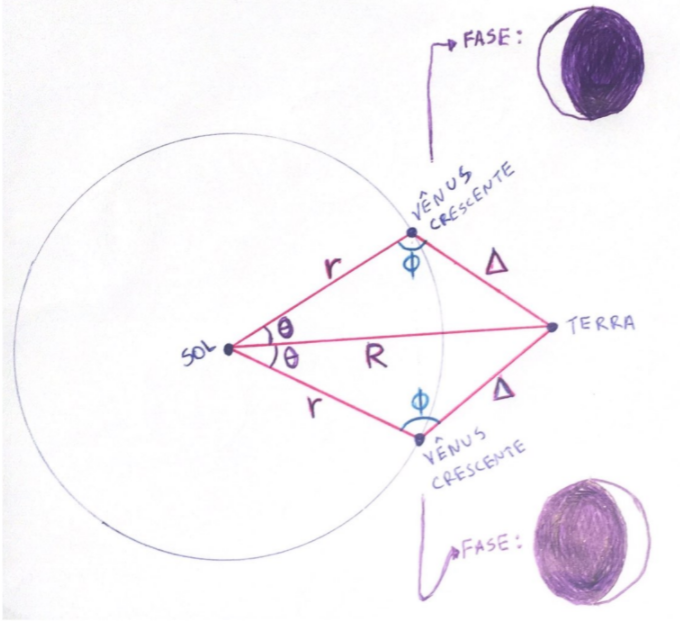
\includegraphics[width=10cm]{01-crescente.PNG}
    
    Figura 1: Fase crescente
\end{center}

\begin{center}
    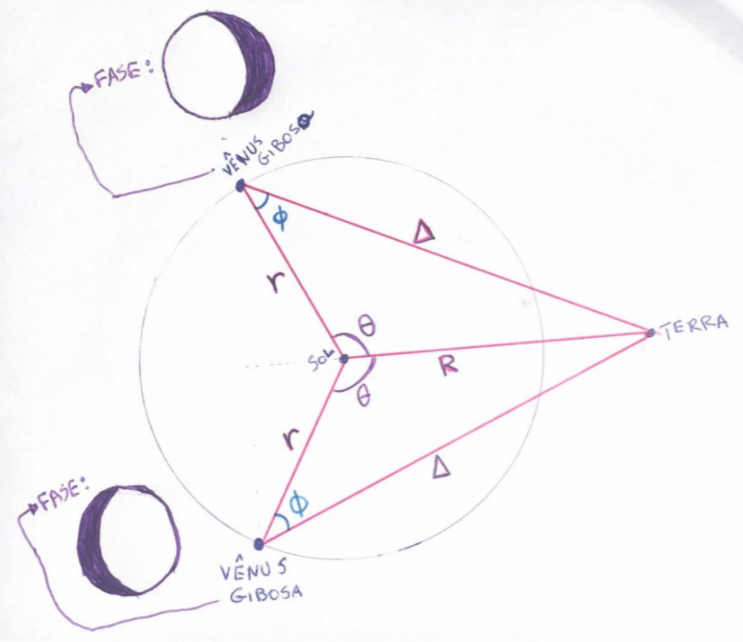
\includegraphics[width=10cm]{02-gibosa.PNG}
    
    Figura 2: Fase gibosa
\end{center}

Nas relações abaixo $R$ e $r$ são constantes e considerados como dados do problema. Utilizando a \textbf{Lei dos cossenos} nos triângulos acima podemos derivar diversas relações, entre elas as seguintes:\\

\textbf{Relação \ref{delta_funcao_teta}}:
$$\Delta ^2=r^2+R^2-2rR\cos \left(\theta \right)$$

A distância entre Terra e Vênus como função do ângulo $\theta$ é dada por:

\begin{equation}\label{delta_funcao_teta}
    \boxed{\Delta \left(\theta \right)=\sqrt{r^2+R^2-2rR\cos \left(\theta \right)}}
\end{equation}\\


\textbf{Relação \ref{cosphi_funcao_delta}}:
$$R^2=\Delta ^2+r^2-2r\Delta \cos \left(\phi \right)$$
$$2r\Delta \cos \left(\phi \right)=\Delta ^2+r^2-R^2$$
Então o cosseno do ângulo $\phi$ em função da distância Terra-Vênus é dado por:

\begin{equation}\label{cosphi_funcao_delta}
    \boxed{\cos \left(\phi \right)=\frac{\Delta ^2+r^2-R^2}{2r\Delta }}
\end{equation}


\subsubsection{Diagramas de fases Nova e Cheia de Vênus}

Os casos representados abaixo podem ser vistos como casos especiais. Tratam-se das fases nova e cheia de Vênus. Com o detalhe de que a fase totalmente cheia é apenas teórica, já que Vênus "se esconde atrás" do Sol quando está na conjunção superior. 

\begin{center}
    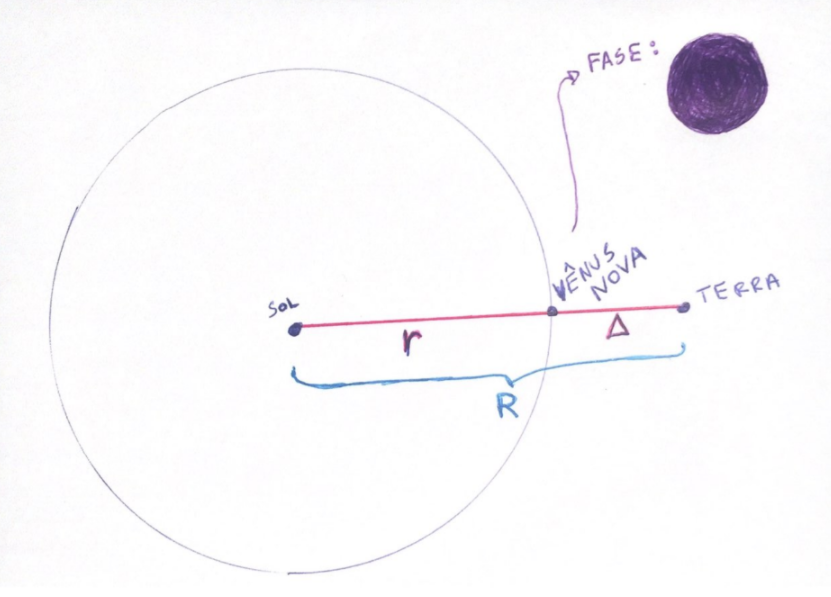
\includegraphics[width=11.5cm]{03-nova.PNG}
    
    Figura 3: Fase nova (Conjunção Inferior)
\end{center}

\begin{center}
    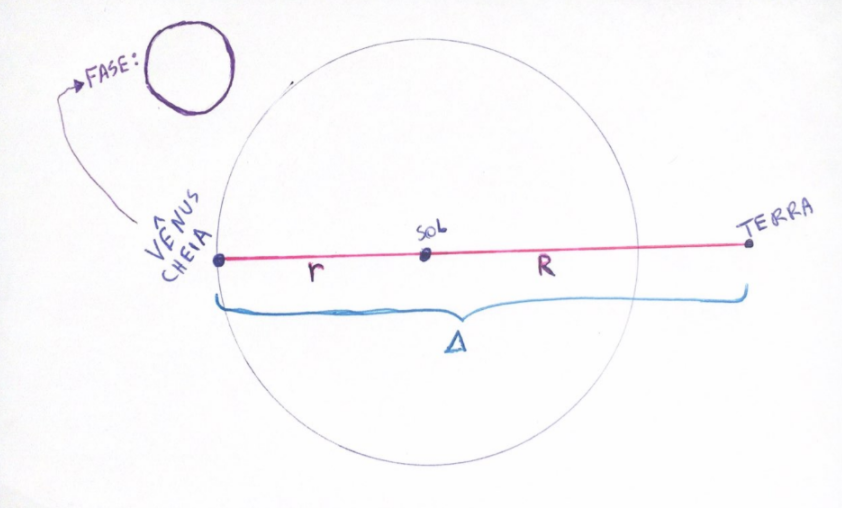
\includegraphics[width=12cm]{04-cheia.PNG}
    
    Figura 4: Fase cheia (Conjunção Superior)
\end{center}

As relações (\ref{delta_funcao_teta}) e (\ref{cosphi_funcao_delta}) encontradas acima também se aplicam aos casos de fase nova e cheia, caso consideremos que $\theta=0$ e $\phi=\pi$ para Vênus na conjunção inferior; e que $\theta=\pi$ e $\phi=0$ quando Vênus está na conjunção superior. Veja:\\

\textbf{Conjunção Inferior} ($\theta=0$ e $\phi=\pi$):

Usando a relação (\ref{delta_funcao_teta}) tem-se:

$$\Delta \left(0 \right)=\sqrt{r^2+R^2-2rR\cos \left(0 \right)}$$
$$\Delta =\sqrt{r^2+R^2-2rR\cdot(1)}$$
$$\Delta ^2=r^2+R^2-2rR$$
$$\Delta ^2=\left(r-R\right)^2$$
$$\Delta =\mid r-R\mid \ \longrightarrow \ R>r\ \longrightarrow \boxed{\Delta =R-r}$$

Usando a relação (\ref{cosphi_funcao_delta}) tem-se:

$$\cos \left(\pi \right)=\frac{\Delta ^2+r^2-R^2}{2r\Delta }$$
$$-1=\frac{\Delta ^2+r^2-R^2}{2r\Delta }$$
$$-2r\Delta =\Delta ^2+r^2-R^2$$
$$R^2=\Delta ^2+r^2+2r\Delta $$
$$R^2=\left(\Delta +r\right)^2\longrightarrow \boxed{R\ =\Delta +r}$$\\ \\


\textbf{Conjunção Superior} ($\theta=\pi$ e $\phi=0$):

Usando a relação (\ref{delta_funcao_teta}) tem-se:

$$\Delta \left(\pi \right)=\sqrt{r^2+R^2-2rR\cos \left(\pi \right)}$$
$$\Delta =\sqrt{r^2+R^2-2rR\cdot(-1)}$$
$$\Delta ^2=r^2+R^2+2rR$$
$$\Delta ^2=\left(r+R\right)^2\longrightarrow \boxed{\Delta =r+R}$$


Usando a relação (\ref{cosphi_funcao_delta}) tem-se:

$$\cos \left(0 \right)=\frac{\Delta ^2+r^2-R^2}{2r\Delta }$$
$$1=\frac{\Delta ^2+r^2-R^2}{2r\Delta }$$
$$2r\Delta =\Delta ^2+r^2-R^2$$
$$R^2=\Delta ^2+r^2-2r\Delta $$
$$R^2=\left(\Delta -r\right)^2\longrightarrow \Delta >r\longrightarrow \boxed{R=\Delta -r}$$

\subsubsection{Valores de $\Delta$ que fazem sentido}
Como visto nos casos extremos acima, os únicos valores fisicamente possíveis para $\Delta$ são tais que: $R-r<\Delta <R+r$. 

Portanto, já que $R>r$, qualquer função em $\Delta$ deve ter domínio: $\left[R-r{,}R+r\right]$.


\subsection{Geometria da Fase $p$ de Vênus}
Nesta seção calcularemos a porcentagem da área da circunfêrencia (visão a partir da Terra) de Vênus que é iluminada pelo Sol. A esta porcentagem se da o nome de \textbf{fase}.

\subsubsection{O $p$ como função de $\phi$: prova para Vênus crescente ($\frac{\pi }{2}<\phi \le \pi$)}

\textbf{Vista de Cima:}\\

Abaixo é mostrada uma ilustração com vista de cima do plano Sol-Vênus-Terra de quando Vênus está em fase crescente. O setor circular $DCA'$ na figura representa a vista de cima da parte que é iluminada pelo Sol e visível pela Terra. Este setor é delimitado por $DC$, que é perpendicular à reta que une o centro de Vênus ao centro da Terra, e por $A'C$ que é perpendicular à reta que une o centro de Vênus ao Sol.

\begin{center}
    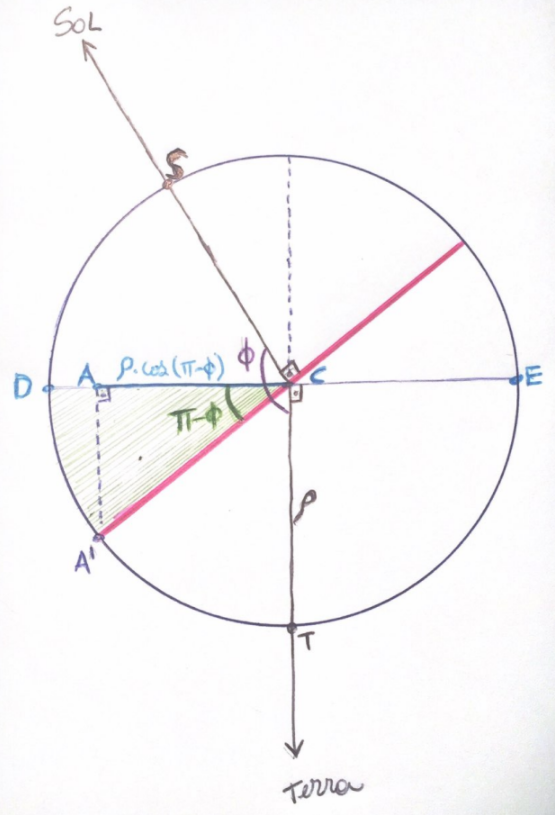
\includegraphics[width=8cm]{05-crescente-de-cima.PNG}
    
    Figura 5: Vênus - vista de cima do plano Sol-Vênus-Terra - crescente
\end{center}

Como pode-se constatar, o ângulo $\hat{ACA'}$ é dado por $\pi-\phi$, e sendo o raio de Vênus igual a $\rho$, então a medida do seguimento $AC$ é $\rho \cos \left(\pi -\phi \right)$.

\textbf{Vista da Terra:}\\
Já a figura abaixo ilustra a mesma situação, só que do ponto de vista de um observador localizado na Terra. 
Como pode-se constatar, a medida $AC=\rho \cos \left(\pi -\phi \right)$ é a metade do eixo menor de uma elipse. A metade desta Elipse é representada por $NASCN$.
\begin{center}
    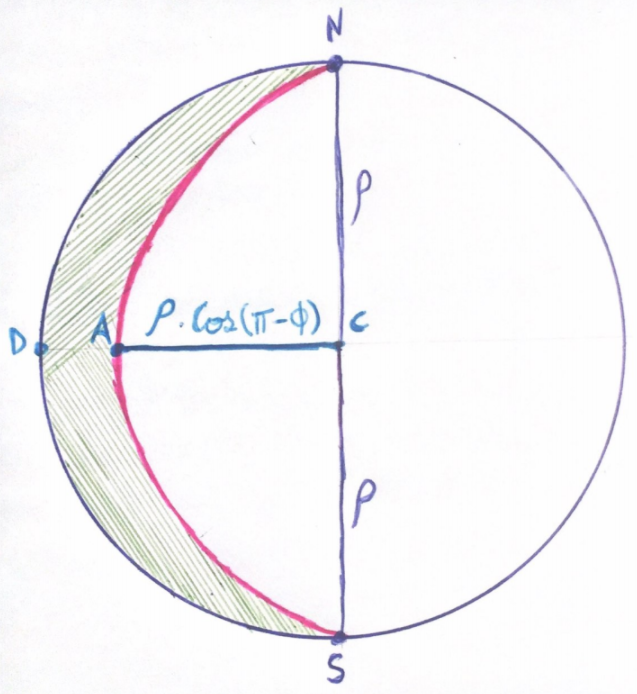
\includegraphics[width=9cm]{06-crescente-elipse.PNG}
    
    Figura 6: Vênus vista da terra - crescente
\end{center}

Vista da Terra, a região iluminada pelo sol é $NDSAN$, e sua área é calculada subtraindo-se a área da meia-circunferência $NDSCN$ pela área da meia elipse $NASCN$. Tem-se então:

$$Area\left(NDSAN\right)=Area\left(NDSCN\right)-Area\left(NASCN\right)$$
$$Area\left(NDSAN\right)=\frac{1}{2}\pi \rho ^2-\frac{1}{2}\pi \rho ^2\cos \left(\pi -\phi \right)$$

Sendo $\cos \left(\pi -\phi \right)=-\cos \left(\phi \right)$, então:

$$Area\left(NDSAN\right)=\frac{1}{2}\pi \rho ^2+\frac{1}{2}\pi \rho ^2\cos \left(\phi \right)$$

Portanto, a área da região iluminada é dada por: 
$$Area\left(NDSAN\right)=\frac{1}{2}\pi \rho ^2\ \left(1+\cos \left(\phi \right)\right)$$

Sendo a área da circunferência completa dada por $\pi \rho ^2$, então para o caso de Vênus crescente \textbf{a fase de Vênus como função de $\phi$ é}:

$$p\left(\phi \right)=\frac{Area\left(NDSAN\right)}{\pi \rho ^2}=\frac{\frac{1}{2}\pi \rho ^2\left(1+\cos \left(\phi \right)\right)}{\pi \rho ^2}$$

$$
    \boxed{p\left(\phi \right)=\frac{1}{2}\left(1+\cos \left(\phi \right)\right)}
$$


\subsubsection{$p$ como função de $\phi$: prova para Vênus gibosa ($0\le \phi \le \frac{\pi }{2}$)}

Pelo mesmo raciocínio utilizado anteriormente, através do esquema abaixo verifica-se que o seguimento $AC$ para o caso da fase gibosa tem medida igual a $\rho \cos \left(\phi \right)$.



\begin{center}
    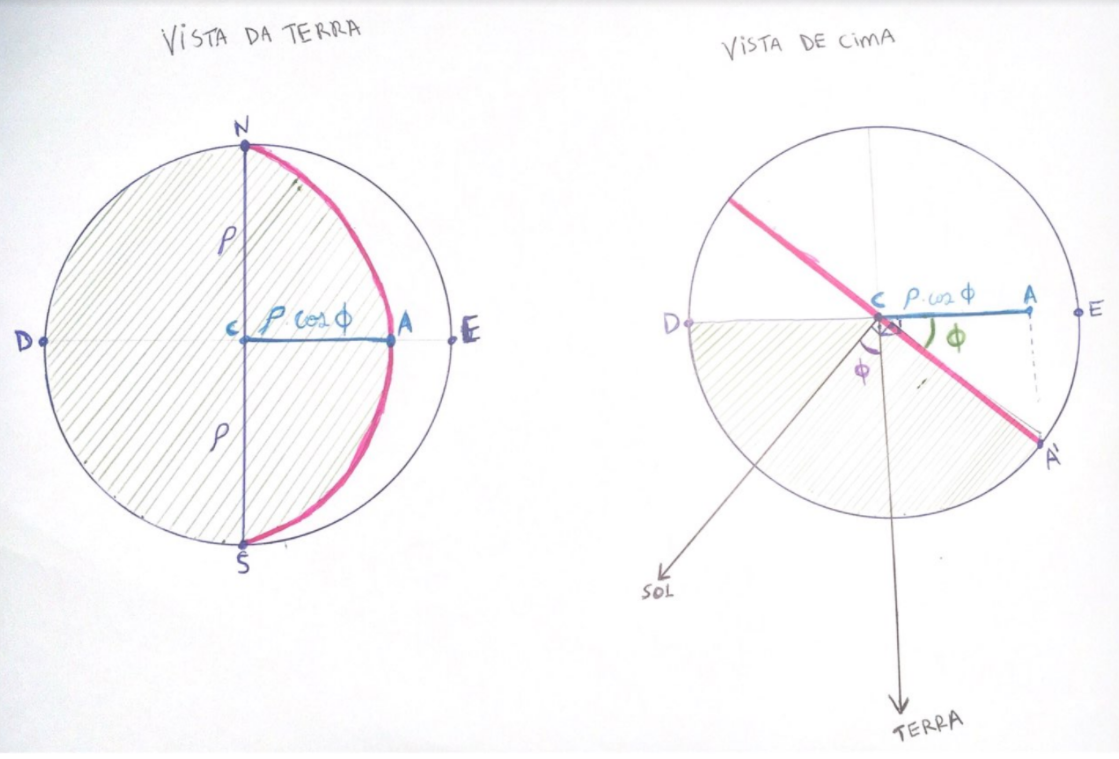
\includegraphics[width=16cm]{07-gibosa-fase.PNG}
    
    Figura 7: Vênus gibosa - Vista da Terra e de cima.
\end{center}

Então, neste caso, a área da região iluminada destacada acima $NDSAN$ é dada pela soma da área da meia circunferência $NDSCN$ com a área da meia elipse $NASCN$. Portanto:

$$Area\left(NDSAN\right)=Area\left(NDSCN\right)+Area\left(NASCN\right)$$
$$Area\left(NDSAN\right)=\frac{1}{2}\pi \rho ^2+\frac{1}{2}\pi \rho ^2\cos \left(\phi \right)$$

Do mesmo modo que no caso de Vênus crescente, a área da região iluminada é dada por: 
$$Area\left(NDSAN\right)=\frac{1}{2}\pi \rho ^2\ \left(1+\cos \left(\phi \right)\right)$$

E portanto, pode-se concluir que \textbf{em todos os casos a fase de Vênus em função de $\phi$ é}:

\begin{equation}\label{fase_funcao_phi}
    \boxed{p\left(\phi \right)=\frac{1}{2}\left(1+\cos \left(\phi \right)\right)}
\end{equation}

\subsubsection{$p$ como função de $\Delta$}

Substituindo a relação (\ref{cosphi_funcao_delta}) no resultado (\ref{fase_funcao_phi}) encontrado acima, tem-se:

$$p\left(\Delta \right)=\frac{1}{2}\left(1+\frac{\Delta ^2+r^2-R^2}{2r\Delta }\right)$$

Portando, a fase de Vênus como função da distância $\Delta$ entre Terra e Vênus é:

\begin{equation}\label{fase_funcao_delta}
    \boxed{p\left(\Delta \right)=\frac{2r\Delta +\Delta ^2+r^2-R^2}{4r\Delta }}
\end{equation}

Mais uma vez, destaca-se que o domínio da função acima é $\left[R-r{,}R+r\right]$. 

\subsubsection{$p$ como função de $\theta$}

Substituindo a relação (\ref{delta_funcao_teta}) no resultado (\ref{fase_funcao_delta}) podemos encontrar $p$ como função de $\theta$. Observe:

$$p\left(\Delta \right)=\frac{2r\Delta +\Delta ^2+r^2-R^2}{4r\Delta }=\frac{1}{2}\left(1+\frac{\Delta ^2+r^2-R^2}{2r\Delta }\right)$$
$$p\left(\theta \right)=\frac{1}{2}\left(1+\frac{\left(\sqrt{r^2+R^2-2rR\cos \left(\theta \right)}\right)^2+r^2-R^2}{2r \sqrt{r^2+R^2-2rR\cos \left(\theta \right)}}\right)\ $$
$$p\left(\theta \right)=\frac{1}{2}\left(1+\frac{r^2+R^2-2rR\cos \left(\theta \right)+r^2-R^2}{2r\sqrt{r^2+R^2-2rR\cos \left(\theta \right)}}\right)\ $$
$$p\left(\theta \right)=\frac{1}{2}\left(1+\frac{2r^2-2rR\cos \left(\theta \right)}{2r\sqrt{r^2+R^2-2rR\cos \left(\theta \right)}}\right)\ $$

Por fim, temos:

\begin{equation}\label{fase_funcao_teta}
    \boxed{p\left(\theta \right)=\frac{1}{2}\left(1+\frac{r-R\cos \left(\theta \right)}{\sqrt{r^2+R^2-2rR\cos \left(\theta \right)}}\right)\ }
\end{equation}



\subsubsection{Fase de Vênus quando $\theta=\pi /2$}

Como exemplo, para encontrar a porcentagem da área da circunferência (vista da Terra) de Vênus que está iluminada pelo sol quando $\theta=\pi /2$, basta substituirmos este valor na função $p\left(\theta \right)$ mostrada em (\ref{fase_funcao_teta}). Tem-se então:

$$p\left(\frac{\pi }{2}\right)=\frac{1}{2}\left(1+\frac{r-R\cos \left(\frac{\pi }{2}\right)}{\sqrt{r^2+R^2-2rR\cos \left(\frac{\pi }{2}\right)}}\right)$$
$$p\left(\frac{\pi }{2}\right)=\frac{1}{2}\left(1+\frac{r-R\cdot \left(0\right)}{\sqrt{r^2+R^2-2rR\cdot \left(0\right)}}\right)$$
$$p\left(\frac{\pi }{2}\right)=\frac{1}{2}\left(1+\frac{r}{\sqrt{r^2+R^2}}\right)$$

Considerando que os raios de órbita de Vênus e da Terra são $r=10.81\times 10^7km$ e $R=14.95\times 10^7km$, então:

$$p\left(\frac{\pi }{2}\right)=\frac{1}{2}\left(1+\frac{10.81\times 10^7}{\sqrt{\left(10.81\times 10^7\right)^2+\left(14.95\times 10^7\right)^2}}\right)$$
$$\boxed{p\left(\frac{\pi }{2}\right)=0.7930}$$

Portanto, quando $\theta=\pi /2$, a circunferência de Vênus vista da Terra está $79.30\%$ iluminada.

\subsection{Discussão sobre o domínio de $p\left(\phi \right)$ e $p\left(\theta \right)$}
Como mostrado nas fuguras de 1 a 4, $\phi$ e $\theta$ são ângulos internos de um triângulo. Como tal, devem estar no intervalo (considerando as conjunções): $0\le\phi,\ \theta\le\pi$.

A partir daqui, poderíamos supor o domínio das funções $p\left(\phi \right)$ e $p\left(\theta \right)$ como $[0,\ \pi]$ e considerar cada metade (os dois triâgulos, o superior e o inferior nas figuras) do movimento relativo de Vênus individualmente.

Porém, como $p\left(\phi \right)$ e $p\left(\theta \right)$ são funções trigonométricas que têm o componente $cos\left(x \right)$, podemos considerar que qualquer ângulo fora do intervalo $[0,\ \pi]$ seja na realidade uma representação do seu correspondente no intervalo $[0,\ \pi]$. Podemos fazer isso pois $\cos \left(\pi +x\right)=\cos \left(\pi -x\right)$, ou também $\cos \left(x\right)=\cos \left(-x\right)$.

Portanto, também poderíamos considerar que o domínio das funções $p\left(\phi \right)$ e $p\left(\theta \right)$ é $\mathbb{R}$ e que ambas têm período $2\pi$, o mesmo período da função $cos\left(x \right)$, mas com o cuidado de que no momento de interpretar estes ângulos, fazer a conversão para seus correspondentes nos 1º e 2º quadrantes, de modo que $cos\left(x_1 \right)=cos\left(x_2 \right)$, sendo $x_1$ um ângulo no intervalo $[0,\ \pi]$, e $x_2$ um ângulo qualquer fora deste mesmo intervalo.

Ao longo do texto adotaremos a interpretação que for mais conviniente em cada caso.

Com estas ressalvas, se considerarmos domínio em $\mathbb{R}$, $p\left(\phi \right)$ e $p\left(\theta \right)$ tem o mesmo período de $\cos \left(x\right)$ e estão representadas abaixo.

\begin{center}
    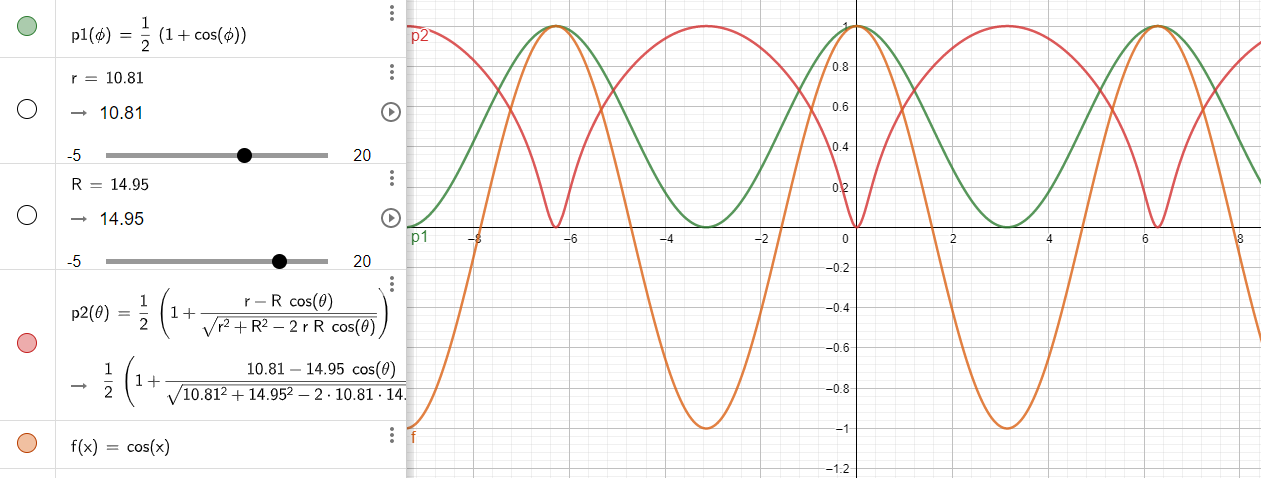
\includegraphics[width=16cm]{08-funcoes-cosseno.PNG}
    
    Figura 8: $p\left(\phi \right)$ e $p\left(\theta \right)$ tem o mesmo período de $\cos \left(x\right)$, caso domínio em $\mathbb{R}$.
\end{center}

A mesma figura foi criada em python com a biblioteca Matplotlib \citep{Biblioteca_Matplotlib}, colocando o eixo x em função de $\pi$ para ficar mais claro que a variação da fase de Venus ocorre no domínio entre 0 e $\pi$

% tirei do texto, pois alterou o modo como tava referenciando nas outras referências... nao sei pq

\begin{lstlisting}[language=Python, caption=Dominio de $\theta$, label=listing_grafico1_mpl] 

import numpy as np
import matplotlib.pyplot as plt
from math import pi as pi

r = 10.81e7
R = 14.95e7

x = np.arange(-2*pi,2*pi,0.1)
y = np.cos(x)
plt.figure(figsize=(12,9))

plt.plot(x/pi,y, 'c:',label='cos')

pt = []
for i in x:
  pt = np.append(pt,p_t(i,r,R))
plt.plot(x/pi,pt, 'r-',label='$p(\\theta)$')

z = 0.5*(1+np.cos(x))
plt.plot(x/pi,z,'g-',label='$p(\phi)$')  

#Melhoramentos do Grafico
plt.title('Comparacao do Dominio de $p(\phi)$ e $p(\\theta)$\nCom a funcao cosseno', fontsize=20)
plt.xlabel('Angulo ($\pi$)',fontsize=15)
plt.ylabel('area da circunferencia de Venus \nvista da Terra ',fontsize=15)
plt.axis([-2.1, 2.1, -1.2, 1.2])
ax = plt.gca()
ax.grid(True)
ax.axhline(0, color='black', lw=2.5)
ax.axvline(0, color='black', lw=2.5)
plt.legend(loc='best',bbox_to_anchor=(0.14, 0.25),fontsize=12)
# remove the frame of the chart
for spine in plt.gca().spines.values():
  spine.set_visible(False) 

plt.savefig('Dominio.png')

\end{lstlisting}

\begin{center}
    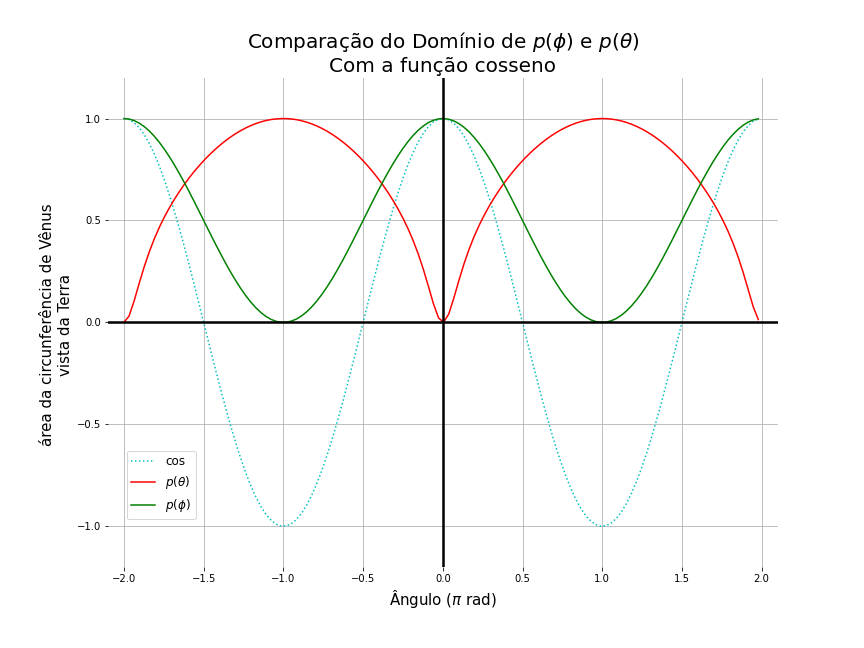
\includegraphics[width=16cm]{10-Dominio.png}
    
    Figura 9: $p\left(\phi \right)$ e $p\left(\theta \right)$ tem o mesmo período de $\cos \left(x\right)$, caso domínio em $\mathbb{R}$.
\end{center}

\section{Propondo um modelo}

Como discutido anteriormente, foram feitas as suposições de que as \textbf{órbitas são circulares e coplanares}.

Para a determinação do momento em que ocorre o brilho máximo serão levadas em consideração os dois fatores seguintes:

\begin{itemize}
  \item O brilho de Vênus visto da Terra é \textbf{diretamente proporcional} à sua fase $p$. 
  \item O brilho de Vênus visto da Terra é \textbf{inversamente proporcional ao quadrado} da distância entre Terra e Vênus ($\Delta$).
\end{itemize}

Dicutiremos agora a validade destas considerações e introduziremos uma constante $K$, para que as proporcionalidades sejam convertidas em uma função matemática.

\subsection{O brilho é diretamente proporcional a $p$}

Considerar que o brilho é proporcional a $p$ é o mesmo que dizer que, tudo o mais constante, quanto maior a porcentagem da área de Vênus (vista da Terra) que é iluminada pelo sol, maior será o brilho. O que parece ser uma consideração válida, já que a área de Vênus que reflete em direção à Terra os raios luminosos vindos do sol aumenta.

Então, sendo o brilho de Vênus denotado por $B$ podemos escrever que:

\begin{equation}\label{brilho_proporcional_p}
    B\propto p
\end{equation}

Substituindo a expressão (\ref{fase_funcao_phi}) em (\ref{brilho_proporcional_p}) então:

$$B\propto \frac{1}{2}\left(1+\cos \left(\phi \right)\right)$$
$$B\propto 1+\cos \left(\phi \right)$$

Desta forma, com todas as considerações feitas, pode-se afirmar que \textbf{o brilho é proporcional a $1+\cos \left(\phi \right)$}.

\subsection{O brilho é inversamente proporcional a $\Delta ^2$}

Como ilustrado na imagem abaixo \citep{site_nasa_imagem_distancia}, a intensidade (ou o \textbf{brilho}) de uma fonte de luz diminui com o inverso do quadrado da distância entre a fonte de luz e o observador.

\begin{center}
    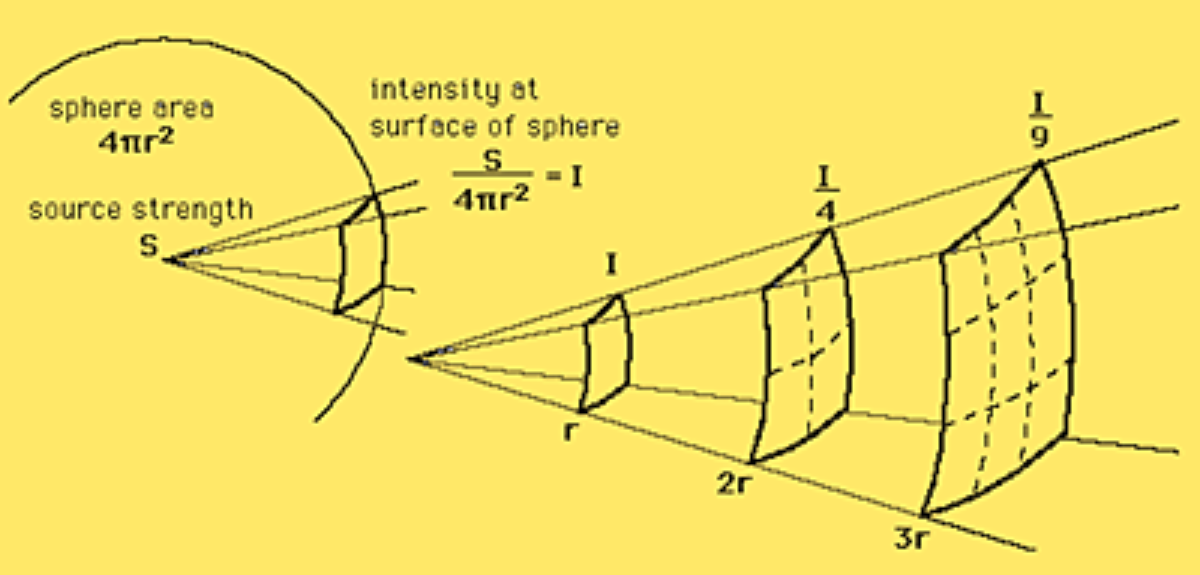
\includegraphics[width=13cm]{09-nasa-distancia.PNG}
    
    Figura 10: Crédito NASA. Intensidade (brilho) diminui pelo inverso do quadrado da distância.
\end{center}

Portanto, de fato podemos considerar que:

\begin{equation}\label{brilho_inverso_deltaquadrado}
    B\propto \frac{1}{\Delta ^2}
\end{equation}

\subsection{Convertendo a proporcionalidade em igualdade}

Juntando os efeitos das relações (\ref{brilho_proporcional_p}) e (\ref{brilho_inverso_deltaquadrado}) tem-se:

\begin{equation}\label{brilho_prop_completo}
    B\propto \frac{p}{\Delta ^2}
\end{equation}

Para que a relação (\ref{brilho_prop_completo}) acima se torne uma igualdade deve-se adicionar uma constante de proporcionalidade. \textbf{Seja esta constante $k_0$}, então a nossa igualdade se torna:

\begin{equation}\label{brilho_igualdade_completo}
    \ \boxed{\ B=k_0\cdot \frac{p}{\Delta ^2}\ }
\end{equation}

Portanto, temos uma igualdade matématica que envolve o brilho de Vênus ($B$), a fase de Vênus ($p$) e a distância entre a Terra e Vênus ($\Delta$). 

Podemos manipular a igualdade (\ref{brilho_igualdade_completo}) de modo a obtermos uma relação do brilho em função dos ângulos $\theta$ e $\phi$, e também do brilho em função da distância $\Delta$, que será feito a seguir.

\subsection{Brilho como função da distância Terra-Vênus ($\Delta$)}

Para que o brilho fique somente em função da variável $\Delta$, devemos substituir a relação (\ref{fase_funcao_delta}) no resultado (\ref{brilho_igualdade_completo}) encontrado acima. Deste modo temos:

$$B\left(\Delta \right)=k_0\cdot \frac{p\left(\Delta \right)}{\Delta ^2}$$
$$B\left(\Delta \right)=k_0\cdot \frac{\frac{2r\Delta +\Delta ^2+r^2-R^2}{4r\Delta }}{\Delta ^2}$$
$$B\left(\Delta \right)=\frac{k_0}{4r}\cdot \frac{2r\Delta +\Delta ^2+r^2-R^2}{\Delta ^3}$$

Como $\frac{k_0}{4r}$ é constante, podemos criar uma nova constante $K$. Então, fazendo $K=\frac{k_0}{4r}$, temos que o brilho em função da distância Terra-Vênus é dado por:

\begin{equation}\label{brilho_funcao_delta}
    \boxed{\ B\left(\Delta \right)=K\cdot \frac{2r\Delta +\Delta ^2+r^2-R^2}{\Delta ^3}\ }
\end{equation}

Como visto anteriormente, o domínio de $B\left(\Delta \right)$ deve ser $\left[R-r{,}R+r\right]$. 

\subsubsection{Discussão sobre a constante de proporcionalidade K}

A introdução da constante de proporcionalidade é apenas um artifício matemático para que convertamos uma relação de proporção em igualdade matemática. Neste caso não nos interessa o valor de $K$, desde que ela seja uma constante positiva, pois queremos apenas estudar com o brilho varia e em que ponto ele é máximo. Diferentes valores de $K$ positivos nos retornarão as mesmas distâncias e ângulos para o brilho máximo, já que dado qualquer $x$, todos os B$\left(x \right)$ estão multiplicados pelo mesmo valor $K$. A utilização de constantes de proporcionalidade é comum em ciências experimentais, e tem a função de "conectar" grandezas que não são naturalmente diretamente relacionadas por uma equação.



\section{Valor de $\Delta$ para brilho máximo}

Para estudar como a função $B\left(\Delta \right)$ varia, calcularemos sua primeira derivada utilizando a regra do quociente.

\subsection{Derivando $B\left(\Delta \right)$}

Então derivando $B\left(\Delta \right)$ tem-se:

$$\frac{dB}{d\Delta }=\frac{\left(2rK+2K\Delta \right)\Delta ^3-\left(2rK\Delta +K\Delta ^2+Kr^2-KR^2\right)3\Delta ^2}{\Delta ^6}$$
$$\frac{dB}{d\Delta }=\frac{K\Delta ^2}{\Delta ^6}\left[\left(2r+2\Delta \right)\Delta -3\left(2r\Delta +\Delta ^2+r^2-R^2\right)\right]$$
$$\frac{dB}{d\Delta }=\frac{K}{\Delta ^4}\left[2r\Delta +2\Delta ^2-6r\Delta -3\Delta ^2-3r^2+3R^2\right]$$

Portanto a primeira derivada de $B\left(\Delta \right)$ é dada por:

\begin{equation}\label{derivada_brilho_em_delta}
    \boxed{\ \frac{dB}{d\Delta }=-\frac{K}{\Delta ^4}\left[\Delta ^2+4r\Delta +3\left(r^2-R^2\right)\right]\ }
\end{equation}

\subsection{Encontrando pontos críticos}

A função $\frac{dB}{d\Delta }$ acima nos mostra, para cada valor de $\Delta$, qual a inclinação da reta tangente à função $B\left(\Delta \right)$.

Como queremos encontrar pontos de máximo na função $B\left(\Delta \right)$, devemos igualar sua primeira derivada a zero. Igualando a zero encontramos os pontos críticos de $B\left(\Delta \right)$, e os pontos de máximo são pontos críticos de uma função.

Fazendo $\frac{dB}{d\Delta }=0$, tem-se:

$$\frac{dB}{d\Delta }=0\ \longleftrightarrow \ \Delta ^2+4r\Delta +3\left(r^2-R^2\right)=0$$

Fazendo Báskara:

$$\Delta =\frac{-4r\pm \sqrt{16r^2-4\cdot \left(1\right)\cdot 3\left(r^2-R^2\right)}}{2\cdot \left(1\right)}$$
$$\Delta =\frac{-4r\pm 2\sqrt{4r^2-3r^2+3R^2}}{2}$$
$$\Delta =-2r\pm \sqrt{r^2+3R^2}$$

Então, caso a função $B\left(\Delta \right)$ tivesse domínio nos $\mathbb{R}$ ela teria dois pontos críticos:\\
$-2r - \sqrt{r^2+3R^2}$ e $-2r + \sqrt{r^2+3R^2}$.

\subsection{Verificando a legitimidade dos pontos críticos}

No nosso caso, $\Delta$ não pode ser negativo, então imediatamente descartamos a solução $-2r - \sqrt{r^2+3R^2}$.

\textbf{Chamaremos a outra solução de}:
\begin{equation}\label{delta_m}
    \boxed{\ \Delta _M=-2r+\sqrt{r^2+3R^2}\ }
\end{equation}

Para verificar se a solução $\Delta _M$ é um ponto crítico aceitável, precisamos provar que ela está dentro do intervalo $[R-r, R+r]$, que é o domínio de $B\left(\Delta \right)$. Fazendo isto temos (considera-se sempre que $R>r$):

Para que a solução satisfaça a condição do domínio, devemos ter:

$$R-r<\Delta _M<R+r$$
$$R-r<-2r+\sqrt{r^2+3R^2}<R+r$$

\textbf{Verificando primeira desiguldadade: ($R-r<\Delta_M$)}

Desenvolvendo temos:

$$R-r<-2r+\sqrt{r^2+3R^2}$$
$$R+r<\sqrt{r^2+3R^2}$$
$$\left(R+r\right)^2<\left(\sqrt{r^2+3R^2}\right)^2$$
$$\left(R+r\right)^2<\sqrt{r^2+3R^2}$$
$$R^2+2Rr+r^2<r^2+3R^2$$
$$2Rr<2R^2$$
$$r<R$$

Portanto, se $r<R$ então $R-r<\Delta_M$. Como estabelecemos que $r<R$, então é verdade que $R-r<\Delta_M$.\\

\textbf{Verificando segunda desiguldadade: ($\Delta_M<R+r$)}

Desenvolvendo temos:

$$-2r+\sqrt{r^2+3R^2}<R+r$$
$$\sqrt{r^2+3R^2}<R+3r$$
$$\left(\sqrt{r^2+3R^2}\right)^2<\left(R+3r\right)^2$$
$$r^2+3R^2<R^2+6Rr+9r^2$$
$$2R^2<6Rr+8r^2$$
$$R^2<3Rr+4r^2$$
$$R^2-3rR-4r^2<0$$

As raízes de $R^2-3rR-4r^2$, supondo $R$ como a variável, são $R=4r$ e $R=-r$. Então:

$$-r<R<4r$$

Fazendo intersecção com o resultado anterior:

$$r<R<4r$$

Transformando a relação anterior temos:

$$r<R\ \longrightarrow \boxed{\frac{r}{R}<1\ }$$
$$R<4r\ \longrightarrow \boxed{\frac{1}{4}<\frac{r}{R}}$$

Assim, para que $\Delta_M$ seja ponto crítico a seguinte relação entre $r$ e $R$ deve ser satisfeita:

$$\boxed{\frac{1}{4}<\frac{r}{R}<1\ }$$

\subsection{Provando que $\Delta _M$ é ponto de máximo}

Queremos provar que $B\left(\Delta \right)$ é crescente para valores um pouco menores que $\Delta _M$, e é decrescente para valores um pouco maiores que $\Delta _M$. Para isso basta analisarmos o sinal de $\frac{dB}{d\Delta }$ em valores de $\Delta$ próximos a $\Delta _M$.

A expressão da derivada de $B\left(\Delta \right)$ é:

$$\frac{dB}{d\Delta }=-\frac{K}{\Delta ^4}\left[\Delta ^2+4r\Delta +3\left(r^2-R^2\right)\right]$$

Fatorando a expressão $\Delta ^2+4r\Delta +3\left(r^2-R^2\right)$, tem-se:

$$\frac{dB}{d\Delta }=-\frac{K}{\Delta ^4}\left[\Delta -\left(-2r-\sqrt{r^2+3R^2}\right)\right]\left[\Delta -\left(-2r+\sqrt{r^2+3R^2}\right)\right]$$
$$\frac{dB}{d\Delta }=-\frac{K}{\Delta ^4}\left(\Delta +2r+\sqrt{r^2+3R^2}\right)\left(\Delta -\Delta _M\right)$$

Como todas as distâncias ($\Delta$, $R$ e $r$) são positivas, a expressão $\Delta +2r+\sqrt{r^2+3R^2}$ é positiva. Designando este fato com um sinal de $\oplus$, temos:


$$\frac{dB}{d\Delta }=-\frac{K}{\Delta ^4}\left(\oplus\right)\left(\Delta -\Delta _M\right)$$

Considerando que $\Delta _M$ as condições vistas anteriormente, então $\Delta _M > 0$. E lembramos que nas considerações abaixo são consideradas \textbf{diferenças infinitesimais} de $\Delta$ em relação a $\Delta_M$. \\

\textbf{Para valores de $\Delta <\Delta _M$}:

Quando $\Delta <\Delta _M\longrightarrow \Delta -\Delta _M<0$, então:

$$\frac{dB}{d\Delta }=-\frac{K}{\Delta ^4}\left(\oplus \right)\left(\ominus \right)\ \longrightarrow \ \frac{dB}{d\Delta }>0$$

\textbf{Para valores de $\Delta >\Delta _M$}:

Quando $\Delta >\Delta _M\longrightarrow \Delta -\Delta _M>0$, então:

$$\frac{dB}{d\Delta }=-\frac{K}{\Delta ^4}\left(\oplus \right)\left(\oplus \right)\ \longrightarrow \ \frac{dB}{d\Delta }<0$$\\

Resumindo os resultados encontrados acima:

$$\Delta <\Delta _M\ \longrightarrow \boxed{\ \frac{dB}{d\Delta }>0\ }$$
$$\Delta >\Delta _M\ \longrightarrow \boxed{\ \frac{dB}{d\Delta }<0\ }$$

\textbf{Assim, $B\left(\Delta \right)$ é crescente antes de $\Delta _M$ e decrescente após $\Delta _M$. Portanto, $\Delta _M$ é de fato um ponto de máximo.}

\subsection{Valor numérico de $\Delta$ tal que $B\left(\Delta \right)$ é máximo}

Agora se tornou trivial calcular o valor da distância entre Terra e Vênus quando o brilho é máximo. Basta substituir os valores de $r=10.81\times 10^7km$ e $R=14.95\times 10^7km$ na expressão de $\Delta_M$, após verificar se $\frac{1}{4}<\frac{r}{R}<1$.

De fato $\frac{1}{4}<\frac{10.81\times 10^7}{14.95\times 10^7}<1\ \longrightarrow \ 0.25<0.72<1$.\\

Substituindo em $\Delta_M$, tem-se:

$$\Delta _M=-2r+\sqrt{r^2+3R^2}$$
$$\Delta _M=\left[-2\left(10.81\right)+\sqrt{\left(10.81\right)^2+3\left(14.95\right)^2}\right]\times 10^7km$$
$$\boxed{\ \Delta _M=6.44\times 10^7km\ }$$

Portanto, a distância entre Terra e Vênus quando o brilho é máximo é de $6.44\times 10^7km$, e ela acontece em dois pontos da trajetória orbital de Vênus em relação a Terra como será ilustrado na seção 8.

\subsection{Gráfico de Brilho máximo em Função de $\Delta$}

Para o Gráfico de Brilho Máximo em Função do Brilho, foi montado um programa simulando o resultado encontrado em (\ref{brilho_funcao_delta}) 
\begin{lstlisting}[language=Python, caption=Brilho de Vênus ($\Delta$), label=listing_B(delta)] 

def BrilhoVenus_d (k,d,r,R): #Brilho de Venus em Funcao da Distancia
  num = 2*r*d+d**2+r**2-R**2
  den = d**3
  b_d = k*num/den
  return b_d

\end{lstlisting}

Tendo a função de Brilho em Função da distância, podemos então criar o código para a geração do gráfico

\begin{lstlisting}[language=Python, caption= Gráfico Brilho de Vênus ($\Delta$), label=listing_grafico_bd] 

import numpy as np
import matplotlib.pyplot as plt

r = 10.81e7
R = 14.95e7
k1 = 12e7
k2 = 15e7
BriV_d1 = [] #vetor para os valores de brilho em funcao da distancia 
BriV_d2 = []

#vetor de valores de distancia entre [R-r,R+r] com 10000 pontos
d = np.arange((R-r),(R+r),21620)
#vetor Brilho(d)
for i in d:
  BriV_d1 = np.append(BriV_d1, BrilhoVenus_d (k1,i,r,R)) #k = 12e7

for i in d:
  BriV_d2 = np.append(BriV_d2, BrilhoVenus_d (k2,i,r,R)) #k = 15e7

plt.figure(figsize=(12,9))
plt.plot(d/10e6,BriV_d1,'g-',label='k = 12 x $10^7$')
plt.plot(d/10e6,BriV_d2,'r-',label='k = 15 x $10^7$')

#Valor maximo de brilho
agmax = BriV_d2.argmax()
dbmax = d[agmax] #64403680.0 km

#Melhoramentos do grafico
ax = plt.gca()
plt.title ('Brilho em Funcao da Distancia ($\\Delta$)\n',fontsize=18)
plt.xlabel('Distancia (Km x $10^7$)',fontsize=14)
plt.ylabel('Brilho (admensional)',fontsize=14)
ax.ticklabel_format(style='sci')
ax.set_xticks([0,3,6.44,10,15,20,25],minor=False)
#ax.xaxis.grid(True, which='minor')
ax.axvline(6.44, linestyle='--', color='k')
#ax.set_yticks([2.77,4.16], minor=True)
#ax.yaxis.grid(True, which='minor')
ax.axhline(BriV_d1[agmax],linestyle='--',color='k')
ax.axhline(BriV_d2[agmax],linestyle='--',color='k')
ax.axhline(0,lw=2.5,color='k')
ax.axvline(0,lw=2.5,color='k')
plt.axis([-0.05, 26, -0.05, 4.3])
plt.legend(bbox_to_anchor=(0.75, 0.5),fontsize=12)
# remove the frame of the chart
for spine in plt.gca().spines.values():
  spine.set_visible(False) 

plt.savefig('Brilho_Distancia.png')

\end{lstlisting}

\begin{center}
    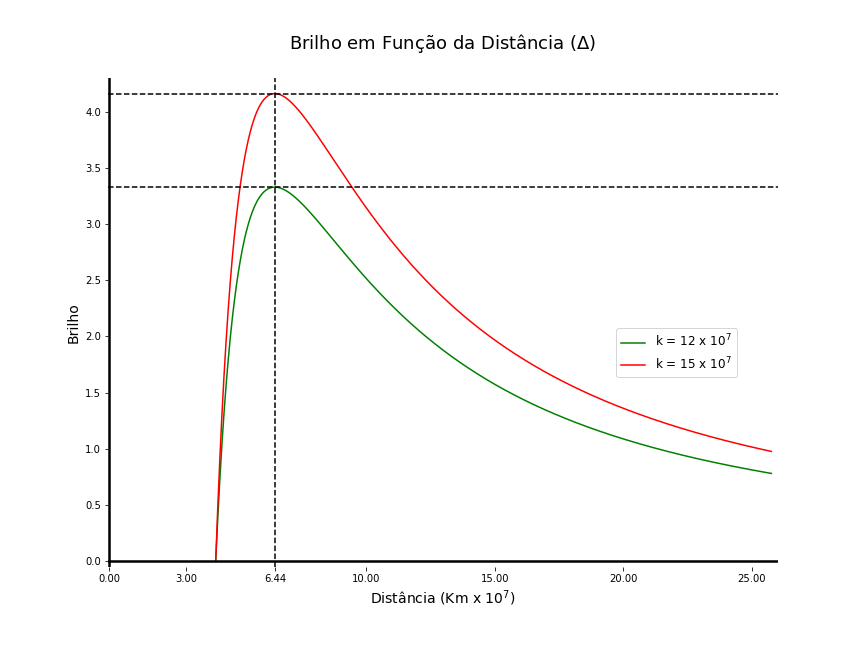
\includegraphics[width=16cm]{11-Brilho_Distancia.png}
    
    Figura 11: Gráfico do Brilho em Função da distância
\end{center}
 
 No gráfico foram colocado duas constantes diferentes para provar empiricamente que o valor de k não afeta a distância onde se tem o brilho máximo.
 
 Também conseguimos o valor simulado de distância 
 
 \begin{center}
    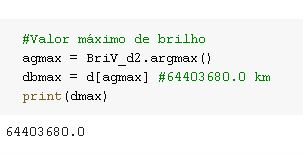
\includegraphics{12-vmax.JPG}
    
    Figura 12: Valor Simulado de distância para Brilho Máximo
\end{center}
  
Na simulação conseguimos o valor de 64403680.0 km, o mesmo valor conseguido teoricamente
r

\section{Distância Terra-Vênus como função de $\theta $}

\subsection{Expressão matemática de $\Delta \left(\theta \right)$}

A expressão (\ref{delta_funcao_teta}) representa a distâcia Terra-Vênus como função de $\theta$, isto é:

$$\Delta \left(\theta \right)=\sqrt{r^2+R^2-2rR\cos \left(\theta \right)}$$

\subsection{Domínio de $\Delta \left(\theta \right)$}
Serão consideradas as mesmas observações feitas para o caso do domínio das funções $p\left(\phi \right)$ e $p\left(\theta \right)$, e se considerará o domínio de $\Delta \left(\theta \right)$ como $\mathbb{R}$, adotando os mesmos cuidados no momento de interpretar os ângulos.

No caso de encontrar o brilho máximo feito abaixo, serão considerados dois triângulos separadamente para considerar todo o movimento relativo de Vênus. O valor de $\theta$ é o mesmo nos dois triangulos, pois são simétricos.

\subsection{Valores de $\theta$ para brilho máximo}

O valor de $\theta$ quando o brilho é máximo é tal que $\Delta \left(\theta \right)=\Delta _M$. Considerando (\ref{delta_funcao_teta}) e (\ref{delta_m}) tem-se então:

$$\Delta \left(\theta \right)=\Delta _M$$
$$\sqrt{r^2+R^2-2rR\cos \left(\theta \right)}=-2r+\sqrt{r^2+3R^2}$$
$$r^2+R^2-2rR\cos \left(\theta \right)=4r^2+r^2+3R^2-4r\sqrt{r^2+3R^2}$$
$$-2rR\cos \left(\theta \right)=4r^2+2R^2-4r\sqrt{r^2+3R^2}$$
$$\cos \left(\theta \right)=\frac{4r^2+2R^2-4r\sqrt{r^2+3R^2}}{-2rR}$$

Neste caso, é suficiente considerarmos  $\theta$ apenas no intervalo $[0,\ \pi]$, então tem-se:

$$\theta =\arccos \left(\frac{4r^2+2R^2-4r\sqrt{r^2+3R^2}}{-2rR}\right)$$

A imagem da função $\arccos \left(\right)$ é $[0,\ \pi]$, condizente com os valores de $\theta$ em um triângulo.
Então, substituindo os valores $r=10.81\times 10^7km$ e $R=14.95\times 10^7km$:

$$\boxed{\ \theta_M =0.39\ rad\ }$$

Na trajetória orbital de Vênus, há duas situações em que $\theta =0.39\ rad$. Ambas estas situações serão ilustradas na seção 8.

\section{Brilho como função de $\theta$}

\subsection{Expressão matemática de $B\left(\theta \right)$}

Para encontrar a expressão do brilho como função de $\theta$, basta substituir (\ref{delta_funcao_teta}) e (\ref{fase_funcao_teta}) em (\ref{brilho_igualdade_completo}):

$$B\left(\theta \right)=k_0\cdot \frac{p\left(\theta \right)}{\left[\Delta \left(\theta \right)\right]^2}$$
$$B\left(\theta \right)=k_0\cdot \frac{\frac{1}{2}\left(1+\frac{r-R\cos \left(\theta \right)}{\sqrt{r^2+R^2-2rR\cos \left(\theta \right)}}\right)}{\left[\sqrt{r^2+R^2-2rR\cos \left(\theta \right)}\right]^2}$$
$$B\left(\theta \right)=\frac{k_0}{2}\cdot \frac{1}{r^2+R^2-2rR\cos \left(\theta \right)}\cdot \left(1+\frac{r-R\cos \left(\theta \right)}{\sqrt{r^2+R^2-2rR\cos \left(\theta \right)}}\right)$$
$$B\left(\theta \right)=\frac{k_0}{2}\cdot \left(\frac{\sqrt{r^2+R^2-2rR\cos \left(\theta \right)}+r-R\cos \left(\theta \right)}{\left[\sqrt{r^2+R^2-2rR\cos \left(\theta \right)}\right]^3}\right)$$

Fazendo $K_1=\frac{k_0}{2}$:


\begin{equation}\label{brilho_funcao_teta}
    \boxed{\ B\left(\theta \right)=K_1\cdot \left(\frac{\sqrt{r^2+R^2-2rR\cos \left(\theta \right)}+r-R\cos \left(\theta \right)}{\left[\sqrt{r^2+R^2-2rR\cos \left(\theta \right)}\right]^3}\right)\ }
\end{equation}


\subsection{Domínio de $B\left(\theta \right)$}
Para o domínio de $B\left(\theta \right)$ são feitas as mesmas considerações para os domínios das outras funções que envolvem angulos neste trabalho. Pode-se considerar o domínio como $\mathbb{R}$, mas com resalvas. Ou podemoms fazer o domínio como $[0,\ \pi]$ e supor dois triângulos, o superior e o inferior (mostrado nas imagens das fases) para considerar o movimento completo.
 
\subsection{Valor da constante de proporcionalidade $K_1$}
Na expressão (\ref{brilho_funcao_teta}) aparece uma constante de proporcionalidade $K_1$. Como foi mostrado nas outras expressões que aparecem constantes de proporcionalidade, não estamos interessados precisamente em seu valor. Já foi verificado que os pontos de máximo não se alteram para valores diferentes dessas constantes. O mesmo acontece com $K_1$.

\subsection{Gráfico de $B\left(\theta \right)$}

Para o gráfico de $B(\theta)$ foi utilizado a mesma função utilizada na criação dos vetores de Brilho em função da distância, porém utilizando $\Delta(\theta)$ descrito em (\ref{delta_funcao_teta}), assim podemos criar os vetores de Brilho em função de $\theta$

\begin{lstlisting}[language=Python, caption=Brilho de Vênus ($\Delta$) e $\Delta(\theta)$, label=listing_B(delta)_(delta_theta] 

def BrilhoVenus_d (k,d,r,R): #Brilho de Venus em Funcao da Distancia
  num = 2*r*d+d**2+r**2-R**2
  den = d**3
  b_d = k*num/den
  return b_d
  
 def Delta_Theta (t,r,R): 

  from math import cos as cos
  from math import sqrt as sqrt
  
  delta = sqrt(r**2+R**2-2*r*R*cos(t))
  return delta

\end{lstlisting}

\subsubsection{Gráfico considerando domínio $[0,\ \pi]$}

Para o gráfico no domínio entre 0 e $\pi$ foi utilizado a biblioteca Matplotlib \citep{Biblioteca_Matplotlib}, com o seguinte código:

\begin{lstlisting}[language=Python, caption=Gráfico Brilho de Vênus ($\theta$), label=listing_grafico_B(theta)] 

#Grafico em funcao de theta
import numpy as np
import matplotlib.pyplot as plt

r = 10.81e7
R = 14.95e7
k1 = 12e7
k2 = 15e7
BriV_t1 = [] #vetor para os valores de brilho em funcao de theta 
BriV_t2 = []

#vetor de valores de distancia entre [0,pi] com 3000 pontos aproximadamente
t = np.arange(0,pi,0.001)

#vetor Brilho(t)
#usando a mesma funcao do Brilho(d), mas usando a funcao delta_theta, para 
#ter delta em funcao de theta
for i in t:
  BriV_t1 = np.append(BriV_t1, BrilhoVenus_d (k1,Delta_Theta(i,r,R),r,R)) #k = 12e7

for i in t:
  BriV_t2 = np.append(BriV_t2, BrilhoVenus_d (k2,Delta_Theta(i,r,R),r,R)) #k = 15e7

plt.figure(figsize=(12,9))
plt.plot(t,BriV_t1,'c-',label='k = 12 x $10^7$')
plt.plot(t,BriV_t2,'m-',label='k = 15 x $10^7$')

#Valor maximo de brilho
agmax = BriV_t2.argmax()
tbmax = t[agmax] #0.391


#Melhoramentos do grafico
ax = plt.gca()
plt.title ('Brilho em Funcao do Angulo ($\\theta$)\n',fontsize=18)
plt.xlabel('$\\theta$(rad)',fontsize=14)
plt.ylabel('Brilho (admensional)',fontsize=14)
ax.set_xticks([0,tbmax,1,1.5,2.0,2.5,3],minor=False)
ax.axhline(BriV_t1[agmax],linestyle='--',color='k')
ax.axhline(BriV_t2[agmax],linestyle='--',color='k')
ax.axvline(tbmax,linestyle='--',color='k')
ax.axhline(0,lw=2.5,color='k')
ax.axvline(0,lw=2.5,color='k')
plt.axis([-0.05, 3.1, -0.05, 4.3])
plt.legend(bbox_to_anchor=(0.95, 0.5),fontsize=12)
# remove the frame of the chart
for spine in plt.gca().spines.values():
  spine.set_visible(False) 

plt.savefig('Brilho_Theta.png')

\end{lstlisting}

\begin{center}
    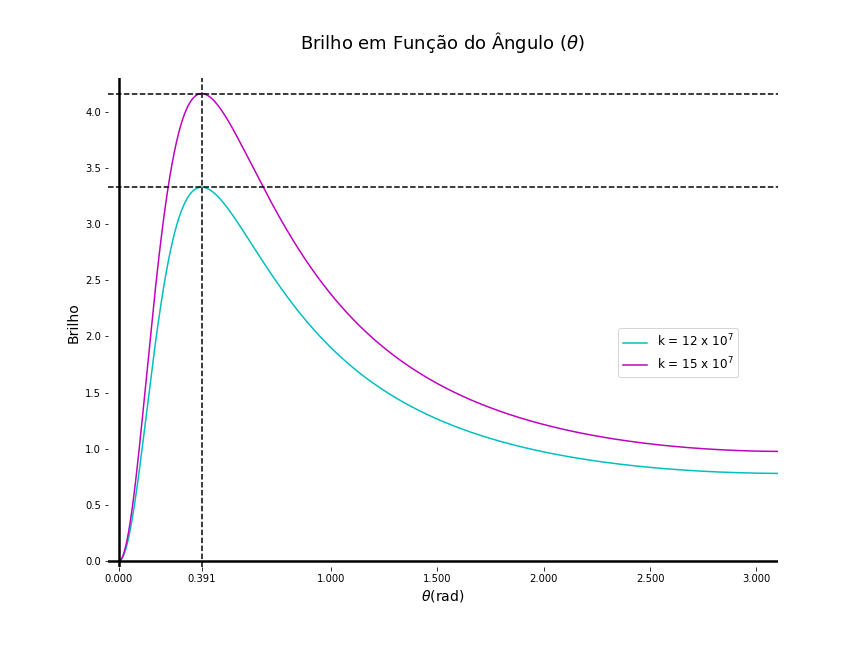
\includegraphics[width=16cm]{13-Brilho_Theta.png}
    
    Figura 13: Gráfico do Brilho em Função do Ângulo Theta [0,$\pi$]
    
\end{center}

No gráfico, foram colocados 2 k's distintos, para demonstrar empiricamente que o ponto de valor de brilho máximo, em função de $\theta$ não depende dessa constante, o gráfico ficou com uma forma bem similar ao brilho em função de $\Delta$, resultado que faz sentido, já que as duas variáveis são interdependentes.

O valor de brilho máximo obtido teoricamente coincide com o simulado no gráfico, no valor de $\theta = 0.391 rad$

\subsubsection{Gráfico considerando domínio $\mathbb{R}$}

Como vimos nas seções anteriores o domínio de $\theta$ e de $\Delta$, são limitados, pois o brilho varia de maneira cíclica. Também vimos que o gráfico do Brilho em função de $\theta$ ou $\Delta$, variam de maneira similar. 
Podemos aumentar o Domínio de $\theta$ para observar graficamente a forma ciclica da Função Brilho($\theta$)

\begin{lstlisting}[language=Python, caption=Gráfico Brilho de Vênus ($\theta$), label=listing_grafico_B(theta)] 

#Grafico em funcao de theta com dominio em R
import numpy as np
import matplotlib.pyplot as plt
from math import pi as pi

r = 10.81e7
R = 14.95e7
k1 = 12e7

BriV_t1 = [] #vetor para os valores de brilho em funcao de theta 

#vetor de valores de distancia entre [2.5pi a 2.5pi] 
t = np.arange(-2.5*pi,2.5*pi,.001)

#vetor Brilho(t)
#usando a mesma funcao do Brilho(d), mas usando a funcao delta_theta, para 
#ter delta em funcao de theta
for i in t:
  BriV_t1 = np.append(BriV_t1, BrilhoVenus_d (k1,Delta_Theta(i,r,R),r,R)) #k = 12e7

plt.figure(figsize=(12,9))
plt.plot(t/pi,BriV_t1,'b-',label='k = 12 x $10^7$')


#Melhoramentos do grafico
ax = plt.gca()
plt.title ('Brilho em Funcao do Angulo ($\\theta$)\n',fontsize=18)
plt.xlabel('$\\theta$($\pi$ rad)',fontsize=14)
plt.ylabel('Brilho (admensional)',fontsize=14)
plt.axis([-2.5, 2.5, -0.05, 3.5])
ax.grid(True)
plt.legend(fontsize=12)

plt.savefig('Brilho_Theta_R.png')

\end{lstlisting}

\begin{center}
    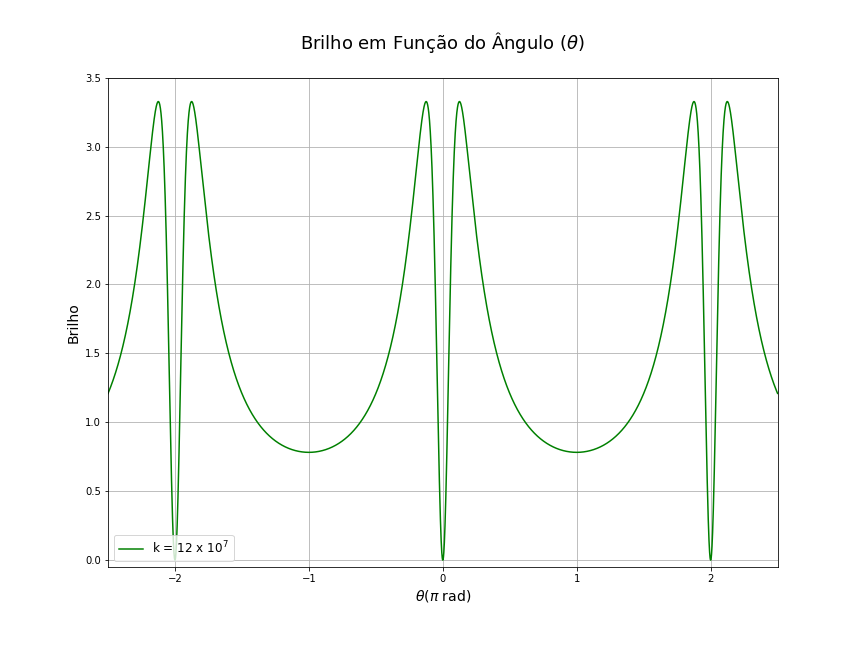
\includegraphics[width=16cm]{14-Brilho_Theta_R.png}
    
    Figura 14: Gráfico do Brilho em Função do Ângulo Theta [-2.5 $\pi$,2.5$\pi$]
    
\end{center}
 
Pelo gráfico da para observar que o ciclo se repete em ciclos de 2$\pi$, porém os valores diferem em ciclos de $\pi$, depois tem uma simetria.

\section{Brilho máximo e Conjunção inferior}

Calcularemos a quantidade de dias antes e depois da conjunção inferior que o brilho é máximo de duas formas diferentes e verifacaremos que elas convergem.

\subsection{Resolução com gravitação universal}

Considerando as órbitas dos planetas circulares, aplicaremos a teoria de \textbf{Gravitação Universal}, em que, consideraremos as velocidades angulares dos planetas constante. Para Vênus e Terra, as velocidades angulares em suas orbitas em torno do sol são: 

$$\begin{matrix}
\boxed{\ \omega _{Terra}=\sqrt{\frac{GM}{R^3}}\ }\ \ \ &\ \ \boxed{\ \omega _{Venus}=\sqrt{\frac{GM}{r^3}}\ }
\end{matrix}$$

Em que $G$ é a constante de gravitação universal, $M$ é a massa do sol, $R$ é o raio de órbita da Terra, e $r$ é o raio de órbita de Vênus.

Assim a velocidade angular relativa entre Vênus e Terra é dada por:

$$\omega _{Rel}=\omega _{Venus}-\omega _{Terra}$$
$$\omega _{Rel}=\sqrt{\frac{GM}{r^3}}-\sqrt{\frac{GM}{R^3}}$$
$$\boxed{\ \omega _{Rel}=\sqrt{GM}\left(\frac{1}{\sqrt{r^3}}-\frac{1}{\sqrt{R^3}}\right)\ }$$\\

Como o ângulo Vênus-Sol-Terra é dado por $\theta$, a variação desse ângulo ($\Delta \theta $) em função de uma variação do tempo ($\Delta t$) é descrita por:

$$\Delta \theta =\omega _{Rel}\cdot \Delta t$$

\begin{equation}\label{teta_horaria}
    \boxed{\ \Delta \theta =\sqrt{GM}\left(\frac{1}{\sqrt{r^3}}-\frac{1}{\sqrt{R^3}}\right)\cdot \Delta t\ }
\end{equation}

Então agora temos uma expressão para relacionar a variação do ângulo $\theta$ com o período de tempo decorrido.

Pelos exercícios anteriores sabe-se que sempre que o ângulo Vênus-Sol-Terra é $\theta = 0.39\ rad$.

Como a conjunção inferior ocorreria quando $\theta$ é zero, isto é $\theta_0=0\ rad$. Então $\Delta \theta$ já está sendo medido em relação à conjunção inferior, e por conseguinte o intervalo de tempo $\Delta t$ é medido em relação a conjunção inferior. 

Sendo:

\begin{itemize}
  \item $G=6.674184\times 10^{-11}\frac{m^3}{kg\cdot s^2}$
  \item $M=1.9891\times 10^{30}kg$
  \item $r=10.81\times 10^7 km$
  \item $R=14.95\times 10^7 km$
\end{itemize}

Substituindo estes dados em (\ref{teta_horaria}) tem-se:

$$\Delta \theta =1.2485\times 10^{-7}\ \frac{rad}{s}\cdot \Delta t$$

Fazendo:

$$\Delta \theta =\theta _M-\theta _0=0.39\ rad\ -\ 0\ rad\ =0.39\ rad$$

Tem-se:

$$0.39\ rad=1.2485\times 10^{-7}\ \frac{rad}{s}\cdot \Delta t$$

Portanto o intervalo de tempo em segundos é:

$$\Delta t=3.127733\times 10^6\ s$$

Sendo $1\ dia = 86400 s$, então:

$$\boxed{\ \Delta t=36.20\ dias\ }$$

Portanto o brilho máximo ocorre no 36º dia após a conjunção inferior, e no 36º dia antes da conjunção inferior. Isto é, quando o ângulo Vênus-Sol-Terra é $\theta_M=0.39\ rad$, que ocorre em dois momentos da trajetório orbital de Vênus, como será ilustrado na seção 8.

\subsection{Resolução com Regra de Três Simples}

Também poderiamos resolver este problema por regra de três. De posse da informação de o intervalo de tempo entre duas conjunções inferiores é de 584 dias, então o intervalo entre a conjunção inferior e superior é de 292 dias, em que $\theta = \pi \ rad$. Portanto:

$$\frac{\Delta \theta }{\Delta t}\ :\ \frac{\pi \ rad }{292\ dias}$$\\

Sabendo que o brilho máximo ocorre quando $\theta_M=0.39\ rad$, tem-se:

$$\frac{0.39\ rad}{\Delta t}\ :\ \frac{\pi \ rad}{292\ dias}\ \ \longrightarrow \ \ \boxed{\ \Delta t=36.24\ dias\ }$$

Portanto encontramos novamente que a quantidade de dias antes e depois da conjunção inferior em que o brilho é máximo é de \textbf{aproximadamente 36 dias} e algumas horas.

\subsection{Precisão das Previsões}

As previsões feitas consideraram que a velocidade angular orbital de cada planeta é constante, e portando considerou que a \textbf{velocidade angular relativa entre eles é constante}. Desse modo, pôde-se estabelecer que que o angulo $\theta$ varia de maneira uniforme com o passar do tempo.

Outro ponto a se ressaltar é sobre as aproximações feitas nas unidades de distância e de massa dos astros, isto é podem sugir problemas ligados à \textbf{escala numérica} ao aproximarmos estes números com ordem de grandeza muito elevada. Assim, pode-se perder um pouco de precisão. Além de termos aproximado o valor do ângulo $\theta$ para o qual o brilho é máximo.


\section{Quando Vênus estará mais brilhante novamente?}

Podemos responder esta pergunta de várias formas. Como foi discutido anteriormente, o brilho de Vênus é máximo quando a distância entre Terra e Vênus é de $\Delta _M=6.44\times 10^7km$ e o ângulo Vênus-Sol-Terra é tem valor $\theta_M =0.39$. E esta situação ocorre duas vezes durante o movimento de Vênus em torno do Sol (imaginando Sol e Terra fixos), cada uma dessas vezes em um dos dois triângulos descritos no início deste trabalho.

E como visto, esta situação ocorre em pouco mais de 36 dias antes e depois da conjunção inferior.

Esta situação está repesentada na figura abaixo:

\begin{center}
    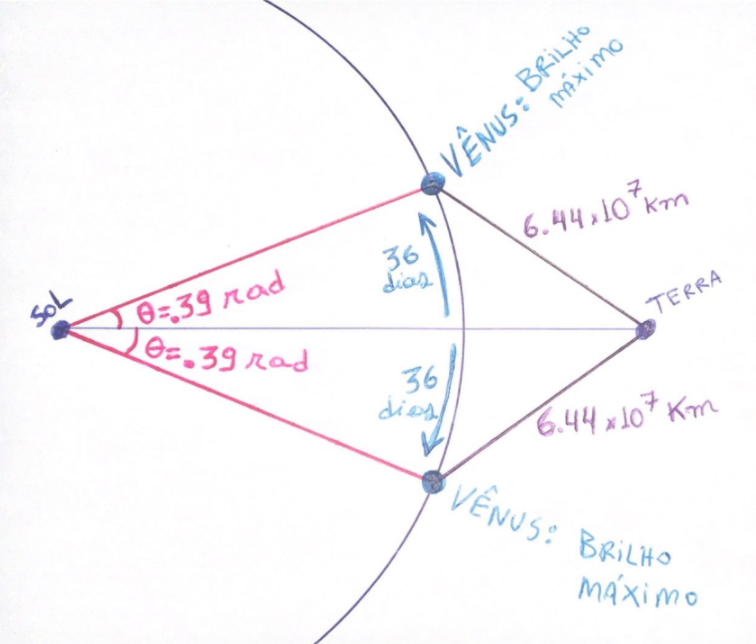
\includegraphics[width=14cm]{15-resumo.PNG}
    
    Figura 15: Resumo das observações deste trabalho.
    
\end{center}

Então: 

\begin{itemize}
  \item Se estamos no ponto de brilho máximo que está 36 dias antes da conjunção inferior, Vênus estará mais Brilhante só daqui a 72 dias.
  \item Se estamos na conjunção inferior, Vênus estará mais brilhante daqui a 36 dias.
  \item Se estamos no ponto de brilho máximo que está 36 dias após a conjunção inferior Vênus só estará mais brilhante daqui a 512 dias ($584 - 72$).
\end{itemize}

Resumindo, vai depender de em que momento da trajetória de Vênus estamos, para saber qual será o próximo ponto de brilho máximo do planeta.

\subsection{Respondendo com base na função $B\left(\theta \right)$ com domínio $\mathbb{R}$}

Como a função é periódica (devido ao termo $\cos \left(\theta \right)$), podemos dizer que os pontos de brilho máximo nesta função ocorrerão sempre que $B\left(x \right) = B\left(0.39\ rad \right)$, pois é $0.39\ rad$ o valor de $\theta$ nos triângulos tal que o brilho é máximo.

Estes pontos de máximo brilho sempre ocorrem quando:
\begin{itemize}
  \item $\theta \approx (0.39 + 2k\pi)\ rad$, $k$ inteiro.
  \item $\theta \approx (-0.39 + 2k\pi)\ rad$, $k$ inteiro.
\end{itemize}



\bibliography{ref.bib}

\end{document}
